%\subsection{Interactive in~transit visualization by staging data in a processing pipeline}

A visualization pipeline is shown in Figure~\ref{part3-ch5-adios:fig:intransitviz}. Pixie3D \cite{ADIOS:Chacon:2002} is a  magneto-hydrodynamic simulation for fusion. This code's output cannot directly be used for visualization because of its internal geometries optimized for execution performance, not for human friendly representation. A separate code, Pixplot, has always been used to process the output on a small number of processes, transform and write the data and multiple meshes in Cartesian coordinates, feasible for visualization. The three components in the visualization pipeline, Pixie3D simulation, Pixplot transformation and ParaView parallel visualization server, represent a typical scenario for concurrent in~transit visualization. Besides the interactive visualization, a light sequential code, Pixmon, is used to extract 2D slices of the original output and to upload images of those slices to a web-accessible dashboard (eSiMon~\cite{ADIOS:Tchoua:cts12}), providing a continuous and remote monitoring of the simulation.


\begin{figure}[h!]
\centering
\myIfColor
{
% use color version
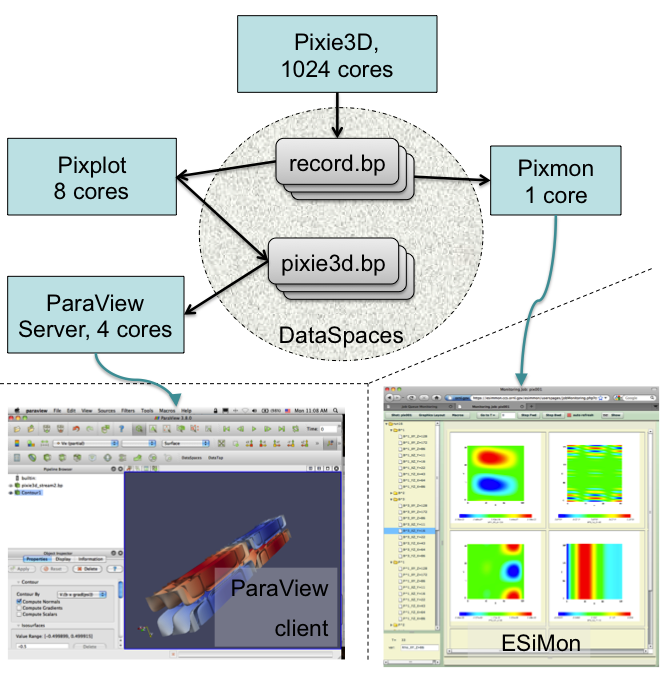
\includegraphics[width=0.5\textwidth]{Chapters/part3-ch5-adios/figs/intransitviz.png}
}
{
% use B&W version
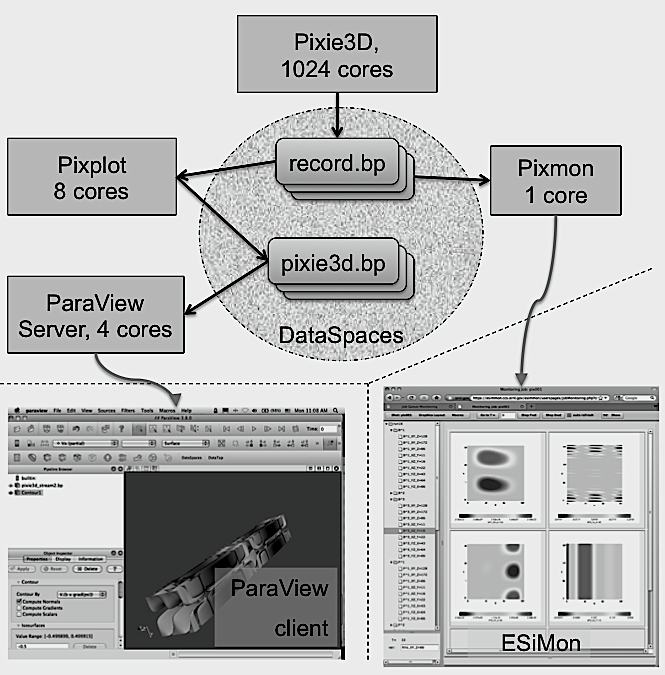
\includegraphics[width=0.5\textwidth]{Chapters/part3-ch5-adios/figs/intransitviz-bw.png}
}
\caption[]
{In~transit analysis and visualization pipeline using ADIOS.
}
\label{part3-ch5-adios:fig:intransitviz}
\end{figure}

The application codes are written as if writing data to files and reading data from files, processing one step at a time and only advancing forward in time. ADIOS allows for a seamless switch from file-based post-processing to online processing helped with memory-to-memory data transfers. Staging methods that transfer data directly from the memory of the producer into the memory of the consumer are best for coupling and for straight analytical pipelines (e.g. DIMES and FlexPath methods of ADIOS). The DataSpaces model~\cite{ADIOS:Docan:cluster12}, however, provides a virtual shared multi-dimensional space using a set of separate nodes as a ``staging area,". Thus multiple, parallel applications can simultaneously read a multi-dimensional array, with an arbitrary decomposition. More importantly for interactive visualization, DataSpaces can hold as many output steps as the allocated memory can hold and can serve a reader with data the producer long has forgotten about. Moreover, DataSpaces provides fault isolation for the application. Failures downstream in a process pipeline does not propagate to the application. More details on using ADIOS and DataSpaces for in-transit visualization can be found in the book on High Performance Visualization~\cite{ADIOS:Bethel-Childs-Hansen:HPV:2012}.
